% Szglab4
% ===========================================================================
%

\chapter{Követelmény, projekt, funkcionalitás}

\thispagestyle{fancy}

\section{Bevezetés}

\subsection{Cél}
A projekt követelményeinek, alapvető felépítésének és funkcionalitásának ismertetése; ezek segítségével körbehatárolni a fejlesztés menetét és a végleges program felépítését, működését. Fejlesztés közben ezeket folyamatosan figyelembe kell majd venni, eltérni tőlük nem szabad.

\subsection{Szakterület}
Az elkészítendő szoftver egy számítógépes játék, így nem egy kifejezett szakterület részére készül, hanem általános felhasználásra, szórakoztatásra. A játék az úgynevezett ``tower defense'' kategóriába sorolható, ezért azoknak ajánlott, akik szeretik az ilyen típusú játékokat.
\subsection{Definíciók, rövidítések}
\comment{A dokumentumban használt definíciók, rövidítések magyarázata.}

\subsection{Hivatkozások}
Szoftver labor 4 - \url{https://www.iit.bme.hu/~szoftlab4/}

\subsection{Összefoglalás}
A dokumentum további részeiben található:
\begin{itemize}
\item Áttekintés, ami nagyvonalakban bemutatja a szoftvert
\item A szoftverrel kapcsolatos követelmények leírása, később ezek figyelembevételével kell a programot fejleszteni
\item Lényegesebb use-case-ek felsorolása
\item Szótár, ami a szoftverrel kapcsolatos nem hétköznapi, illetve nem hétköznapi értelmében használt szavak definícióit tartalmazza
\item A projekt kivitelezésének terve
\item Projekt napló
\end{itemize}

\section{Áttekintés}
\subsection{Általános áttekintés}
\comment{A kialakítandó szoftver legmagasabb szintű architekturális képe. A fontosabb alrendszerek felsorolása, a közöttük kialakítandó interfészek lényege, a felhasználói kapcsolatok alapja. Esetleges hálózati és adattárolási elvárások.}

\section{Áttekintés}
\subsection{Általános áttekintés}
\comment{A kialakítandó szoftver legmagasabb szintű architekturális képe. A fontosabb alrendszerek felsorolása, a közöttük kialakítandó interfészek lényege, a felhasználói kapcsolatok alapja. Esetleges hálózati és adattárolási elvárások.}

\begin{samepage}
A szoftver legmagasabb szintű architekturális képe:
\newline
\begin{figure}
\centering
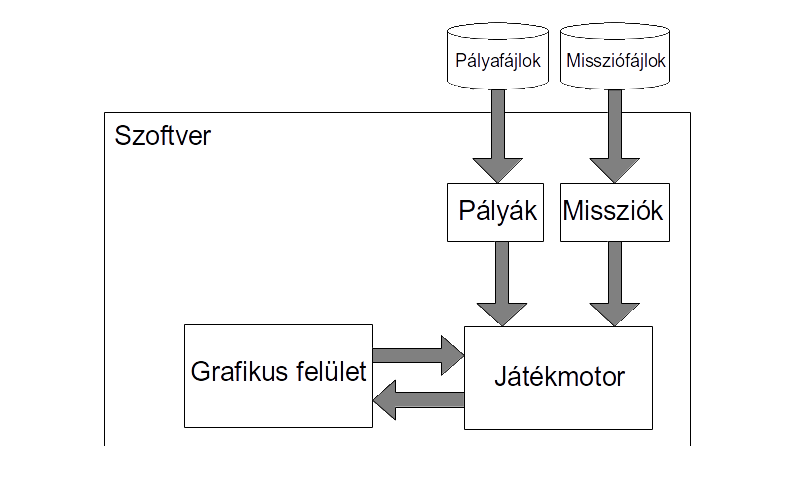
\includegraphics[width=170mm]{images/architekturalis_kep.png}
\caption{Architekturalis kep}
\label{overflow}
\end{figure}
\end{samepage}
\newline
Hálózatot a szoftver egyáltalán nem használ. Háttértáron pedig a program saját fájljai - .jar archivum(ok), a kirajzoláshoz szükséges képek, és az egyes pályákat, valamint missziókat tároló fájlok - számára kell helyet biztosítani. Ezeken kívül nincs további futási idejű tárhelyigénye.

\subsection{Funkciók}
\comment{A feladat kb. 4000 karakteres (kb 1,5 oldal) részletezettségű magyar nyelvű leírása. Nem szerepelhetnek informatikai kifejezések.}



\subsection{Felhasználók}
\comment{A felhasználók jellemzői, tulajdonságai}

\subsection{Korlátozások}
\comment{Az elkészítendő szoftverre vonatkozó – általában nem funkcionális - előírások, korlátozások.}

\subsection{Feltételezések, kapcsolatok}
\comment{A dokumentumban használt anyagok, web-oldalak felsorolása}

\section{Követelmények}
\subsection{Funkcionális követelmények}


% \comment{Az alábbi táblázat kitöltésével készítendő. Dolgozzon ki követelmény azonosító rendszert! Az ellenőrzés módja szokásosan bemutatás és/vagy kiértékelés. Prioritás lehet alapvető, fontos, opcionális. Az alapvető követelmények nem teljesítése végzetes. Forrás alatt a követelményt előíró anyagot, szervezetet kell érteni. Esetünkben forrás lehet maga a csapat is, mikor ő talál ki követelményt. Use-case-ek alatt az adott követelményt megvalósító használati esete(ke)t kell megadni.}

% Azonosító, Leírás, Ellenőrzés, Prioritás, Forrás, Use-case, Komment
\begin{longtable}{| p{16mm} | p{4cm} | l | l | l | p{15mm} | p{2cm} |}
\hline
\textbf{Azonosító}   & \textbf{Leírás} & \textbf{Ellenőrzés} & \textbf{Prioritás} & \textbf{Forrás} & \textbf{Use-case} & \textbf{Komment} \tabularnewline
\hline\hline
1.01 & Tornyokat lehet építeni & bemutatás & alapvető & megrendelő & Torony építése &  \tabularnewline
\hline
1.02 & Az ellenfelek igyekszenek eljutni a célig & bemutatás & alapvető & megrendelő &  & \tabularnewline
\hline
1.03 & A tornyok képesek lőni & bemutatás & alapvető & megrendelő &  &  \tabularnewline
\hline
1.04 & Az ellenfelek sebződnek a tornyok lövedékétől & kiértékelés & alapvető & megrendelő &  &  \tabularnewline
\hline
1.05 & Az ellenfelek bizonyos mértékű sebződés után meghalnak & bemutatás & alapvető & megrendelő &  & \tabularnewline
\hline
1.06 & Az elpusztított ellenfelek után varázserőt kap a játékos & bemutatás & alapvető & megrendelő &  &  \tabularnewline
\hline
1.07 & A különböző ellenfelek, különböző tulajdonságokkal rendelkezeknek & bemutatás & opcionális & csapat &  & Különböző életerő, sebesség \tabularnewline
\hline
1.08 & Vannak utak & bemutatás & alapvető & megrendelő &  &  \tabularnewline
\hline
1.09 & Az ellenfelek az utakról nem térnek le & bemutatás & alapvető & megrendelő &  &  \tabularnewline
\hline
1.10 & Tornyot nem lehet útra építeni & bemutatás & fontos & megrendelő & Torony építése &  \tabularnewline
\hline
1.11 & Akadályokat lehet építeni & bemutatás & alapvető & megrendelő & Akadály építése &  \tabularnewline
\hline
1.12 & Akadályt csak útra lehet rakni & bemutatás & fontos & megrendelő & Akadály építése &  \tabularnewline
\hline
1.13 & Az akadályok lassítják az ellenfeleket & bemutatás & fontos & megrendelő &  &  \tabularnewline
\hline
1.14 & A tornyoknak van tüzelési gyakorisága, hatótávolsága & bemutatás & alapvető & megrendelő &  &  \tabularnewline
\hline
1.15 & Tornyokat és akadályokat varázskövekkel lehet ellátni & bemutatás & alapvető & megrendelő & Torony/ akadály echant-olás &  \tabularnewline
\hline
1.16 & Különböző varázskövek vannak & bemutatás & opcionális & megrendelő &  &  \tabularnewline
\hline
1.17 & Idővel egyre gyakrabban érkeznek ellenfelek, egyre nagyobb csoportban & bemutatás & fontos & megrendelő &  &  \tabularnewline
\hline
1.18 & A játékot el lehet indítani & bemutatás & alapvető & megrendelő & Új játék indítása &  \tabularnewline
\hline
1.19 & A játékot fel lehet adni & bemutatás & opcionális & csapat & Feladás &  \tabularnewline
\hline
1.20 & Több pálya van & bemutatás & opcionális & csapat & Pálya kiválasztása &  \tabularnewline
\hline
1.21 & A játékból ki lehet lépni & bemutatás & alapvető & csapat & Kilépés &  \tabularnewline
\hline
1.22 & Ha az összes ellenfél meghalt, a játékos nyer & bemutatás & alapvető & csapat &  &  \tabularnewline
\hline
1.23 & Több útvonal vezet a célig & bemutatás & alapvető & csapat &  &  \tabularnewline
\hline
1.24 & Ha egy ellenfél eljut a célig, a játékos veszít & bemutatás & alapvető & csapat &  &  \tabularnewline
\hline
\end{longtable}

\subsection{Erőforrásokkal kapcsolatos követelmények}

% \comment{A szoftver fejlesztésével és használatával kapcsolatos számítógépes, hardveres, alapszoftveres és egyéb architekturális és logisztikai követelmények}

% Azonosító, Leírás, Ellenőrzés, Prioritás, Forrás, Komment
\begin{longtable}{| l | p{5cm} | l | l | l | l |}
\hline
\textbf{Azonosító}   & \textbf{Leírás} & \textbf{Ellenőrzés} & \textbf{Prioritás} & \textbf{Forrás} & \textbf{Komment} \tabularnewline
\hline\hline
2.01 & Git &  & alapvető & csapat & Elosztott verziókezelő \tabularnewline
\hline
2.02 & Github account &  & alapvető & csapat & Git tárhely \tabularnewline
\hline
2.03 & JRE6 &  & alapvető & megrendelő & \tabularnewline
\hline
2.04 & Eclipse &  & opcionális & csapat & Java IDE \tabularnewline
\hline
2.05 & IntelliJ IDEA &  & opcionális & csapat & Java IDE \tabularnewline
\hline
2.06 & HSZK-ban találhatókkal azonos vagy jobb teljesítményű PC &  & alapvető & megrendelő &  \tabularnewline
\hline
2.07 & Monitor &  & alapvető & csapat &  \tabularnewline
\hline
2.08 & Egér &  & alapvető & csapat &  \tabularnewline
\hline
2.09 & Enterprise Architect &  & opcionális & csapat & UML modellező \tabularnewline
\hline
2.10 & TeXworks &  & opcionális & csapat & LaTeX editor \tabularnewline
\hline
\end{longtable}


\subsection{Átadással kapcsolatos követelmények}
% \comment{A szoftver átadásával, telepítésével, üzembe helyezésével kapcsolatos követelmények}

% Azonosító, Leírás, Ellenőrzés, Prioritás, Forrás, Komment
\begin{longtable}{| l | p{5cm} | l | l | l | l |}
\hline
\textbf{Azonosító}   & \textbf{Leírás} & \textbf{Ellenőrzés} & \textbf{Prioritás} & \textbf{Forrás} & \textbf{Komment} \tabularnewline
\hline\hline
3.01 & Szkeleton átadás & bemutatás & alapvető & megrendelő & márc. 26. \tabularnewline
\hline
3.02 & Proto átadás & bemutatás & alapvető & megrendelő & ápr. 23. \tabularnewline
\hline
3.03 & Teljes program átadása & bemutatás & alapvető & megrendelő & máj. 14. \tabularnewline
\hline
3.04 & Útmutató alapján telepíthető, külső segítség nélkül & bemutatás & fontos & megrendelő &  \tabularnewline
\hline
3.05 & A programnak működnie kell a BME HSZK számítógépein & bemutatás & alapvető & megrendelő &  \tabularnewline
\hline
\end{longtable}

\subsection{Egyéb nem funkcionális követelmények}
\comment{A biztonsággal, hordozhatósággal, megbízhatósággal, tesztelhetőséggel, a felhasználóval kapcsolatos követelmények}

Nincs egyéb nem funkcionális követelmény.

% Azonosító, Leírás, Ellenőrzés, Prioritás, Forrás, Komment
% \begin{longtable}{| l | l | l | l | l | l |}
% \hline
% \textbf{Azonosító}   & \textbf{Leírás} & \textbf{Ellenőrzés} & \textbf{Prioritás} & \textbf{Forrás} & \textbf{Komment} \tabularnewline
% \hline\hline
% 4.01 & ... &  & alapvető & megrendelő & ... \tabularnewline
% \hline
% \end{longtable}


\section{Lényeges use-case-ek}
% \comment{A 2.3.1-ben felsorolt követelmények közül az alapvető és fontos követelményekhez tartozó használati esetek megadása az alábbi táblázatos formában.}

\subsection{Use-case leírások}

\usecase
{Új játék indítása}
{Új játék indul el}
{Játékos}
{1. A játékos kiválasztja a menüben az ``Új játék'' feliratú gombot, és megnyomja. \newline
2. Ezután kiválaszthatja  a nehézséget és a pályát. \newline
3. Elindul a játék a kiválasztott pályával és nehézséggel.}

\usecase
{Pálya kiválasztása}
{Ki kell választani a pályát amelyen játszani kíván.}
{Játékos}
{Új játék indítása után egy listából ki kell választani a pályát amelyen játszani kíván.}

\usecase
{Nehézségi szint kiválasztása}
{Ki kell választani, hogy milyen nehézségen kíván játszani.}
{Játékos}
{Új játék indítása, és a pálya kiválasztása után, ki kell választani három opció közül,
 hogy mennyire legyen a játék nehéz.}

\usecase
{Torony építése}
{Új tornyot épít}
{Játékos}
{Olyan mezőre kattintva, ahol nincsen út vagy torony, ott új torony épül,
ha van elég varázserő hozzá.}

\usecase
{Akadály építése}
{Új akadályt épít}
{Játékos}
{Olyan mezőre kattintva ahol út van, és még nincsen akadály, ott akadály épül,
ha van elég varázserő hozzá.}

\usecase
{Torony/akadály enchant-olás}
{Már létező tornyot vagy akadályt enchant-olunk}
{Játékos}
{Toronyra vagy akadályra kattintva ki kell választani, hogy milyen drágakővel szeretné enchant-olni,
és ha van elég varázserő hozzá akkor megtörténik az enchant.}

\usecase
{Feladás}
{Feladjuk a jelenlegi játékot}
{Játékos}
{A feladás gombra kattintva a játék végetér, és megnyílik a főmenü.}

\usecase
{Kilépés}
{Kilép az alkalmazásból}
{Játékos}
{Az ablak jobb felső sarkában, a bezárásra kattintva az alkalmazás kilép.}

\subsection{Use-case diagram}

\begin{figure}[ht!]
\centering
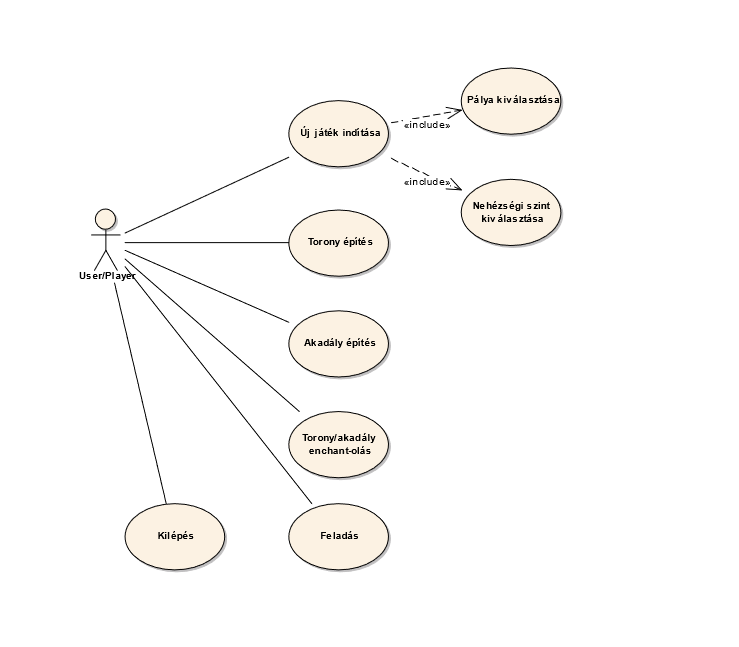
\includegraphics[width=170mm]{images/UseCase.png}
\caption{Use-case diagram}
\label{overflow}
\end{figure}

\section{Szótár}
\comment{A szótár a követelmények alapján készítendő fejezet. Egy szótári bejegyzés definiálásához csak más szótári bejegyzések és köznapi – a feladattól független – fogalmak használhatók fel. A szótár mérete kb. 1-2 oldal legyen.}

\section{Projekt terv}
% \comment{Tartalmaznia kell a projekt végrehajtásának lépéseit, a lépések, eredmények határidejét, az egyes feladatok elvégzéséért felelős személyek nevét és beosztását, a szükséges erőforrásokat, stb. Meg kell adni a csoportmunkát támogató eszközöket, a választott technikákat! Definiálni kell, hogy hogyan történik a dokumentumok és a forráskód megosztása!}

\subsection{Csapat}
A csapat 4 főből áll. A feladatokat úgy próbáljuk kiosztani, hogy lehetőleg mindenkinek azonos nehézségű feladat jusson, miközben a személyes preferenciáit is betartjuk.

\begin{longtable}{| l | p{7cm} | l | l | l | l |}
\hline
\textbf{Név} & \textbf{Felelősségek} \tabularnewline
\hline\hline
\adam & UML, dokumentáció \tabularnewline
\hline
\antal & Kód, dokumentáció \tabularnewline
\hline
\bator (csapatvezető) & Menedzsment, kód \tabularnewline
\hline
\torok & Dokumentáció, kód \tabularnewline
\hline

\end{longtable}

\subsection{Kommunikáció}

\textbf{Verziókezelés} Mivel többen dolgozunk a projekten, ezért fontos, hogy mindig mindenkinek elérhető legyen a legfrissebb forráskód, illetve dokumentáció. Ezért valamilyen módon meg kell osztanunk egymással az elkészített dokumentumokat, programkódokat. Erre a Git elosztott verziókezelő szoftvert választottuk. Ehhez a központi tárhelyet a Github biztosítja. \\
Azért esett erre a megoldásra a választás, mert így könnyen tudjuk követni ki mit csinált, egyszerűen tudunk visszaállni egy korábbi verzióra és közösen meg tudjuk vitatni, hogy mely változások kerüljenek be a végleges projektbe.
Mind a programkódot, mind a dokumentációt verziózzuk, az utóbbi azért tehető meg, mert TeX-et használunk a dokumentáció készítéséhez, aminek a forrásfájlai sima szöveges dokumentumok.
\\ \\
\textbf{Wiki}
A Githubnak van egy wiki szolgáltatása, ahová feladatkiosztásokat és egyéb fontos tudnivalókat rakunk fel. \\ \\
\textbf{Facebook}
A csapatnak létrehoztunk egy privát Facebook csoportot, ahová a csapat bármely tagja írhat bejegyzéseket, illetve hozzászólhat bejegyzésekhez. \\ \\
\textbf{Megbeszélések}
Továbbá hetente (ha szükség van rá) tartunk egy konferenciabeszélgetést, ahol megbeszéljük ki hol tart a munkájában, milyen problémák és kérdések merültek fel. Ehhez a Skype nevű programot használjuk. \\
Ezeken kívül minden héten találkozunk a kijelölt konzultáció időpontban, szerdánként 8:15-kor.

\subsection{Használt programok}
\textbf{Verziókezelés}
A verziókezeléshez a feljebb bővebben kifejtett Git-et használjuk. \\ \\
\textbf{Dokumentáció}
A dokumentációhoz a TeXworks szoftvert használjuk. Ezzel könnyen lehet .tex fájlokat szerkeszteni és ezekből dokumentumot generálni. \\
A dokumentációban található UML diagrammok készítéséhez az Enterprise Architect nevű szoftvert használjuk. \\ \\
\textbf{Fejlesztőkörnyezet}
A forráskódot Eclipse, illetve IntelliJ IDEA nevű fejlesztőkörnyezetekben készítjük.

\subsection{Mérföldkövek, határidők}
\begin{longtable}{| l | p{7cm} | l | l | l | l |}
\hline
\textbf{Dátum} & \textbf{Leírás} & \textbf{Ellenőrzés} \tabularnewline
\hline\hline
2014.02.24. & Követelmény, projekt, funkcionalitás & beadás \tabularnewline
\hline
2014.03.03. & Analízis modell kidolgozása 1. & beadás \tabularnewline
\hline
2014.03.10. & Analízis modell kidolgozása 2. & beadás \tabularnewline
\hline
2014.03.17. & Szkeleton tervezése & beadás \tabularnewline
\hline
2014.03.24. & Szkeleton & beadás \tabularnewline
\hline
2014.03.26. & Szkeleton & bemutatás \tabularnewline
\hline
2014.03.31. & Prototípus koncepciója & beadás \tabularnewline
\hline
2014.04.07. & Részletes tervek & beadás \tabularnewline
\hline
2014.04.22. & Prototípus & beadás \tabularnewline
\hline
2014.04.23. & Prototípus & bemutatás \tabularnewline
\hline
2014.05.12. & Grafikus változat & beadás \tabularnewline
\hline
2014.05.14. & Grafikus bemutató & bemutatás \tabularnewline
\hline
2014.05.16. & Összefoglalás & beadás \tabularnewline
\hline
\end{longtable}


